\documentclass[titlepage]{article}
\usepackage{polski}
\usepackage[utf8]{inputenc}
\usepackage{enumitem}
\usepackage{graphicx}
\usepackage{placeins}
\usepackage{listings}
\usepackage{booktabs}
\usepackage{listings}
\lstset{breaklines}
\lstset{captionpos=b}   % podpis pod listingiem

\title{System do wyszukiwania tras biegowych/rowerowych/turystycznych na podstawie opisów ze stron WWW}
\author{Jakub Guzek, Paweł Kamiński, Jan Muczyński}

\usepackage{natbib}
\usepackage{graphicx}

\begin{document}

\maketitle

\section{Treść zadania}
Celem zadania jest stworzenie systemu pozwalającego wyszukać trasy do uprawiania sportów takich jak np. bieganie czy kolarstwo. Trasy powinny być znajdywane na stronach WWW w czasie działania programu. Na potrzeby projektu rozważane są tylko opisy w języku angielskim.

\section{Opis projektu}
Projekt ma na celu znajdowanie na podstawie analizy tekstów znalezionych na stronach internetowych, które są podobne do opisów ścieżek sportowych, na których podstawie został wyuczony model klasyfikacyjny. Teksty pochodziły między innymi ze stron blogów, serwisów turystycznych czy biur podróży. System posiada plik konfiguracyjny ze zdefiniowaną listą stron internetowych, na których wyszukiwane były teksty przez specjalnie do tego zaimplementowane crawlery. Treści tekstów są poddawane analizie z wykorzystaniem algorytmu \textit{Doc2Vec}, aby ocenić czy są odpowiedniej kategorii. Teksty, które zostały pozytywnie sklasyfikowane trafiają następnie do bazy danych.
Użytkownik wpisuje zapytanie o ścieżkę do uprawiania sportu w programie. Jest ono następnie przetwarzane przez system i porównywane z zebranymi tekstami w bazach danych. Jeśli tekst pasuje do wpisanego zapytania to jest wyświetlany użytkownikowi.


\section{Użyte narzędzia}
Projekt został zaimplementowany w języku Java, przy wykorzystaniu frameworka Akka. Do budowy projektu wykorzystywany jest \textit{Maven}. Przy implementacji crawlera, użyty został \textit{crawler4j} oraz narzędzie \textit{Selenium}. Do przetwarzania tekstu naturalnego wykorzystywana była biblioteka \textit{deeplearning4j}.

\section{Architektura}
System jest rozproszony, złożony z wielu agentów. Głównym agentem, tworzącym wszystkie inne jest \textit{ConsoleActor}. Przyjmuje on polecenia użytkownika i przekazuje je dalej. Dla każdego serwisu internetowego, z którego pobierane są dane, tworzone są grupy agentów złożone z \textit{SearcherActor}, \textit{CrawlerActor}, \textit{DatabaseActor} oraz \textit{NLPActor}. Grupy służą do wyszukiwania nowych artykułów oraz do ich gromadzenia. \textit{SearcherActor} jest pośrednikiem pomiędzy bazą danych, crawlerem i konsolą. Crawler służy do wyszukiwania nowych informacji o ścieżkach sportowych w internecie. Dla każdego znalezionego tekstu uruchamia \textit{NLPActora}, który potrafi przetworzyć język naturalny i sklasyfikować taki dokument. Jeśli dokument został pozytywnie sklasyfikowany to wstawiany jest do bazy danych. Baza danych korzysta z \textit{NLPActorów} natomiast do porównywania zapytania wprowadzonego przez użytkownika ze zgromadzonymi tekstami.

\subsection{Aktorzy}

W tabeli \ref{table:actors} zostali wymienieni aktorzy występujący w zaimplementowanym systemie.

\begin{table}[h]
\centering
\begin{tabular}{@{}cc@{}}
\toprule
\textbf{Nazwa aktora}              & \textbf{Opis}                                                                                                                                                                                                                                                                                                                                         \\ \midrule
\multicolumn{1}{c|}{ConsoleActor}  & \begin{tabular}[c]{@{}c@{}}Główny aktor, który tworzy wszystkich innych aktorów.\\ Reprezentuje konsolę umożliwiającą na interakcję \\ z użytkownikiem.\\ Zaimplementowany jako maszyna stanowa, posiadająca \\ dwa stany: oczekiwanie na działanie użytkownika \\ oraz stan oczekiwania na uzyskanie\\ odpowiedzi od potomnych agentów.\end{tabular} \\ \midrule
\multicolumn{1}{c|}{CrawlerActor}  & \begin{tabular}[c]{@{}c@{}}Aktor przemierzający strony w poszukiwaniu \\ interesujących artykułów. Tworzony przez SearcherActora. \\ Korzysta z NLPActora do klasyfikacji napotkanych tekstów.\end{tabular}                                                                                                                                           \\ \midrule
\multicolumn{1}{c|}{DatabaseActor} & \begin{tabular}[c]{@{}c@{}}Aktor reprezentujący bazę danych, w której \\ przechowywane są znalezione informacje \\ o ścieżkach sportowych.\end{tabular}                                                                                                                                                                                               \\ \midrule
\multicolumn{1}{c|}{NLPActor}      & \begin{tabular}[c]{@{}c@{}}Aktor potrafiący przetwarzać język naturalny. \\ Służy do klasyfikacji znalezionych w Internecie tekstów \\ oraz do porównywania nich następnie z zapytaniami użytkownika.\end{tabular}                                                                                                                                    \\ \midrule
\multicolumn{1}{c|}{SearcherActor} & \begin{tabular}[c]{@{}c@{}}Aktor pośredniczący w komunikacji pomiędzy konsolą, \\ crawlerem i bazą danych. Aktorzy tego typu są tworzeni \\ dla każdej strony internetowej z konfiguracji \\ i należą do grupy broadcastowej konsoli. \\ Temu aktorowi podlega crawler oraz baza danych.\end{tabular}                                                 \\ \bottomrule
\end{tabular}
\caption{Aktorzy znajdujący się w systemie}
\label{table:actors}
\end{table}

\FloatBarrier

\subsection{Wiadomości}

W tabeli \ref{table:messages} znajdują się typy wiadomości, które służą do komunikacji pomiędzy aktorami w systemie.

\begin{table}[h]
\centering
\begin{tabular}{@{}c|c|c|c@{}}
\toprule
\textbf{Wiadomość}  & \textbf{\begin{tabular}[c]{@{}c@{}}Aktor \\ źródłowy\end{tabular}} & \textbf{\begin{tabular}[c]{@{}c@{}}Aktor \\ docelowy\end{tabular}} & \textbf{Opis}                                                                                                                                                                                                                      \\ \midrule
PathInfoResponse    & NLPActor                                                           & ConsoleActor                                                       & \begin{tabular}[c]{@{}c@{}}Odpowiedź na zapytanie o ścieżkę \\ przeznaczona dla użytkownika.\\ Jest przekazywana do konsoli \\ w celu wyświetlenia użytkownikowi.\end{tabular}                                                     \\ \midrule
CrawlerStarter      & SearcherActor                                                      & CrawlerActor                                                       & \begin{tabular}[c]{@{}c@{}}Wiadomość uruchamiająca \\ crawling witryny WWW.\end{tabular}                                                                                                                                           \\ \midrule
PathInfoRecord      & NLPActor                                                           & DatabaseActor                                                      & \begin{tabular}[c]{@{}c@{}}Wiadomość przeznaczona \\ dla bazy danych. \\ Zawiera opis znalezionej \\ przez crawler ścieżki,\\  która powinna zostać \\ umieszczona w bazie danych.\end{tabular}                                    \\ \midrule
TextWithQuery       & DatabaseActor                                                      & NLPActor                                                           & \begin{tabular}[c]{@{}c@{}}Wiadomość zawierająca \\ opis ścieżki \\ wraz z zapytaniem użytkownika.\\ Wysyłana do NLPActora \\ w celu określenia \\ w jak dużym stopniu\\ dany tekst spełnia \\ wymagania użytkownika.\end{tabular} \\ \midrule
TextToClassify      & CrawlerActor                                                       & NLPActor                                                           & \begin{tabular}[c]{@{}c@{}}Wiadomość wysyłana przez crawlera \\ do NLPActora \\ w celu sprawdzenia, \\ czy znaleziony tekst \\ opisuje ścieżkę sportową.\end{tabular}                                                              \\ \midrule
SearchPathInfoQuery & ConsoleActor                                                       & DatabaseActor                                                      & \begin{tabular}[c]{@{}c@{}}Wiadomość z zapytaniem \\ użytkownika. \\ Przekazywana do SearcherActora \\ a następnie do bazy danych\\ w celu znalezienia \\ interesujących opisów ścieżek.\end{tabular}                              \\ \bottomrule
\end{tabular}
\caption{Wiadomości wysyłane w systemie}
\label{table:messages}
\end{table}

\FloatBarrier

\begin{figure}[h!]
\centering
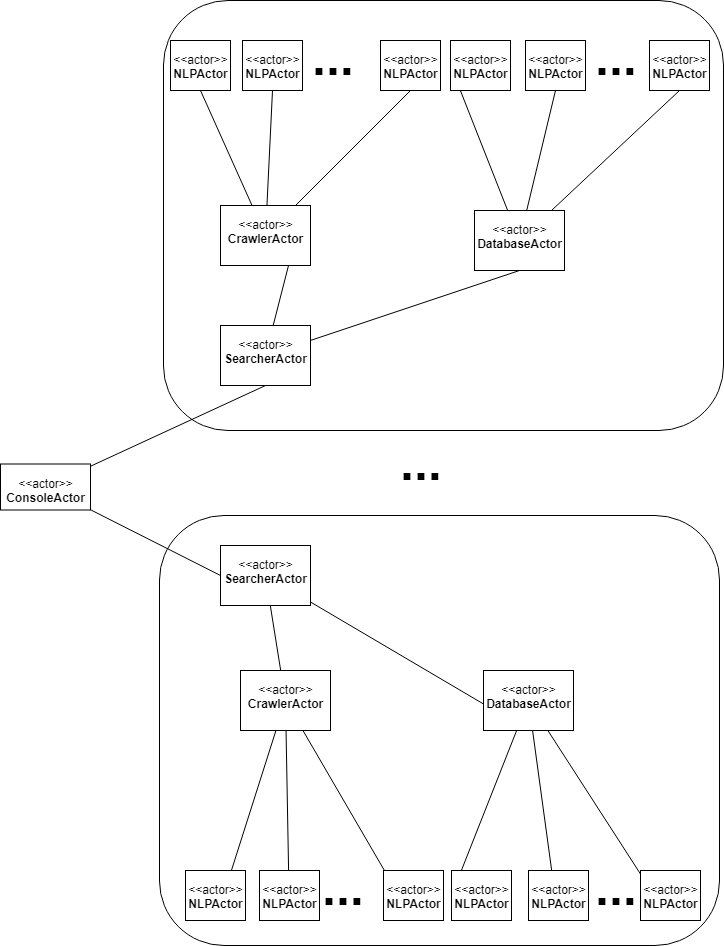
\includegraphics[width=\textwidth]{sag.png}
\caption{Architektura systemu}
\label{fig:architecture}
\end{figure}

\FloatBarrier

\section{Crawler}

Do przeszukiwania stron internetowych w celu pozyskania informacji na temat np. tras biegowych, stworzony został moduł crawlera. Można w nim wyróżnić dwa podmoduły. Jeden jest odpowiedzialny za przeszukiwanie serwisu dostępnego pod podanym adresem URL, aby pozyskać adresy jego podstron, gdzie mogą znajdować się interesujące treści. Drugi podmoduł odwiedza każdy znaleziony adres i pobiera treści potencjalnie niosące wartość z perspektywy użytkownika. Do stworzenia pierwszej części modułu crawlera wykorzystana została biblioteka crawler4j. Umożliwia ona powołanie wiele równoległych obiektów do przeszukiwania podanego serwisu. W trakcie przeszukiwania, odkryte adresy są uznawane za adresy podstron serwisu, jeśli ich domena jest taka, jak domena pierwotnego adresu serwisu. Tak pozyskane adresy są przekazywane do innego obiektu crawlera, który korzysta z narzędzia Selenium, czyli automatycznej przeglądarki. Wykorzystanie Selenium ma na celu podniesienie skuteczności przeszukiwania, ponieważ udostępnia pełnoprawną przeglądarkę (w naszym przypadku Chromium), która jest w stanie możliwie najdokładniej rednerować strony, również takie, których fragmenty są generowane dynamicznie. Przeglądarka po odwiedzeniu każdego adresu, szuka elementów w domie HTML, które zostały zdefiniowane w pliku konifguracyjnym jako takie, które mogą nieść wartościowe treści. W ten sposób pozyskiwane są, za pomocą modułu crawlera, informacje o różnych trasach, które następnie trafiają do modułu odpowiedzialnego, za ich przetwarzanie. 

\section{Przetwarzanie języka naturalnego}
\label{sec:nlp}

Funkcjonalność modułu NLP sprowadzić można do dwóch głównych zadań: klasyfikacja nowych tekstów i szukanie tekstów pasujących do zapytania użytkownika. Pierwsza funkcjonalność jest połączona z działaniem crawlera. Ten, chodząc po stronach, \textit{scrapuje} ich główną zawartość -- treść artykułów. Na ich podstawie moduł NLP musi stwierdzić, czy tekst przedstawia opis ścieżki, czy też nie. Do tego zadania został wykorzystany \textbf{doc2vec}. Jest to złożony algorytm z dziedziny sztucznej inteligencji (przetwarzania języka naturalnego), który z dokumentu (tekstu, paragrafu, zdania, itp.) generuje wektory. Do stworzenia części modułu NLP odpowiedzialnej za to zadanie wykorzystane zostały biblioteki z serii bibliotek deeplearning4j (DL4J). Pierwszym krokiem w realizacji tego zadania było stworzenie modelu (niejako klasyfikatora) i nauczenie go (uczenie nadzorowane). W tym celu należało zebrać korpus. W naszym przypadku był to zbiór tekstów z różnych blogów i tym podobnych, które zawierają opis ścieżek biegowych, rowerowych lub hikingowych. Teksty zebrano z różnych stron -- między innymi z tych, które następnie znajdowały się w configu crawlera, ponieważ treści tamtych artykułów zawierały to, czego szukaliśmy. Do korpusu dodano również dla rozróżnienia teksty z innych dziedzin jak finanse, nauka, czy zdrowie. Ostatecznie więc klasyfikator (model) posiadał aż 6 etykiet: trasy biegowe (running), rowerowe (cycling), hikingowe (hiking) oraz nauka (science), zdrowie (health) i finanse (finance). Wszystkie teksty wraz z ich etykietami zostały podane podczas nadzorowanego nauczania. Nauczony model został zapisany do pliku tak, aby każdy aktor NLP mógł go wczytać i nie tracić czasu na ponowne uczenie. Zadanie samego klasyfikowania nowego tekstu zaczyna się od wygenerowania dla niego wektora \textit{INDArray} (klasa z biblioteki DL4J). Następnie korzystając z biblioteki DL4J można było wyliczyć odległość kosinusową tekstu z każdą z etykiet. Jeśli klasyfikator (model) uznał, że zgodność tekstu i etykiet oryginalnych (ścieżki rowerowe, biegowe, hikingowe) przekroczyła minimalny próg (ustalony empirycznie 0.55), to zostało uznawane, że tekst posiada opis ścieżki. Drugie z głównych zadań polegało na znalezieniu podobieństwa między tekstem a zapytaniem użytkownika. Na początku eksperymenty dotyczyły techniki \textbf{word embedding}. Niestety wykorzystanie algorytmów word2vec i GloVe dawało bardzo słabe wyniki. Było to spowodowane dużymi szumami w wektorach stworzonych na podstawie długich tekstów (w porównaniu do krótkiego zapytania użytkownika). To powodowało, że wektor wygenerowny przez zapytanie ,,knee surgeon near New York'' według odległości kosinusowej był bardziej podobny do tekstu o ścieżce rowerowej we Francji niż wektor wygenerowany przez zapytanie ,,cycling in France''. Przez to zostało stworzone rozwiązanie, które polegało na TF-IDF  (ang. TF – \textit{term frequency}, IDF – \textit{inverse document frequency}). Oczywiście na początku każdy z tekstów zostaje poddany stemmingowi. Od czystego TF-IDF różni się tym, że nie tylko dla każdego wyrazu z zapytania sprawdza się jego współczynnik TF-IDF, ale również dla synonimów wygenerowanych dla każdego słowa z zapytania oraz dla kilkunastu słów bliskich wygenerowanych dla każdego słowa na podstawie algorytmu GloVe. Oczywiście wyrażona liczbowo ,,bliskość'' tekstu do zapytania odpowiednio ważyła synonimy i wyrazy bliskie.
od koniec badań została zauważona jeszcze jedna zależność, a mianowicie można było stworzyć dwa dokumenty -- jeden dla tekstu, a drugi dla zapytania, wykorzystując do tego infrastrukturę (model doc2vec) stworzoną na potrzeby pierwszego zadania. Jak się można było spodziewać dobrze sobie radził z określeniem podobieństwa, jednak przy dłuższych tekstach miał problemy z określeniem sportu. Przy 3 zapytaniach różniących się nazwą sportu dawał bardzo podobne wyniki. 
Ostatecznie trzeba było wybrać jedną z dwóch metod do drugiego zadania, dlatego została wybrana metoda druga, gdyż pojedyncze zapytanie zwracało wyniki w znacznie krótszym czasie. Na pewno sporym minusem jest to, że po zebraniu nowej puli tekstów, należy douczyć (lub nauczyć na nowo, jeśli biblioteka nie pozwala douczać modelu) na podstawie nowych (poprawnie zebranych i zwalidowanych) tekstów. Trzeba to robić, aby rozszerzać słownik i rozszerzać możliwości zbierania nowych tekstów, które nie są podobne (w rozumieniu bliskości tekstów doc2vec) do początkowego korpusu. Rozszerzenie słownika skutkuje także braniem pod uwagę większej ilości nazw własnych, w tym nazwy miejscowości.



\section{Przeprowadzone eksperymenty}
\subsection{Crawler}
Uruchomiony program czytał z pliku konfiguracyjnego strony, które następnie były poddawane crawlingowi w celu wyszukiwania nowych artykułów zawierających ścieżki turystyczne. Teksty znalezione w Internecie były poddawane klasyfikacji w celu sprawdzenia czy są dla nas interesujące. Użytkownik miał możliwość wpisania w konsolę zapytania, które następnie było analizowane i porównywane z tekstami w bazie danych. W taki sposób podczas jednego uruchomienia programu zostało znajdywanych około 200 tekstów. Problemem, którym napotkaliśmy było to, że pomimo otwierania nowych stron co około sekundę, bardzo często serwisy te nas blokowały z powodu zbyt dużego ruchu, który na nie generowaliśmy.

\subsection{Przetwarzanie języka naturalnego}
Testy modułu NLP powinny się zacząć od stworzenia i nauczenia modelu, co powinno być zrobione wcześniej, a zostało już opisane w rozdziale~\ref{sec:nlp}. Pierwsze, co można zbadać w takim modelu to jego zgodność z danymi, na podstawie których się nauczył -- korpusów z etykietami. W tym celu zostały napisane testy pierwszego zadania, czyli klasyfikacji tekstów. Zanim zaczniemy je omawiać, trzeba najpierw przypomnieć jaki jest wynik działania klasyfikatora w tym modelu. Są to pary etykieta plus zgodność tekstu z tą etykietą w skali od -1 do 1. Test polegał na tym, że każdy tekst był klasyfikowany i przyjmował on taką etykietę, z której miał najwyższy wynik. W listingu \ref{lst:nlp-training} (skopiowany z konsoli) widać tabelę, która jest prezentacją wyników tego testu. Etykiety w kolumnach oznaczają prawdziwe etykiety tekstu, który był badany. Rzędy to etykiety, które są wynikiem klasyfikatora (modelu). Idealny wynik testu jest wtedy, kiedy wszystkie liczy oprócz przekątnej (tu: z lewego górnego rogu do prawego dolnego rogu) to zera. Listing \ref{lst:nlp-training} prezentuje właśnie taką sytuację, co pokazuje, że model poprawnie się nauczył.

\begin{lstlisting}[frame=single,
stepnumber=1,
numbersep=10pt,
tabsize=4,
showspaces=false,
showstringspaces=false,
label=lst:nlp-training,
caption=Wynik testu dla tekstów treningowych]
		cycling	hiking	running	finance	health	science	
cycling	21		0		0		0		0		0		
hiking	0		29		0		0		0		0		
running	0		0		17		0		0		0		
finance	0		0		0		10		0		0		
health	0		0		0		0		10		0		
science	0		0		0		0		0		10			
\end{lstlisting}

Ciekawszym przypadkiem jest test podobny do poprzedniego z taką różnicą, że teksty zostały pobrane z różnych źródeł (zescrapowane teksty i zebrane ręcznie). Są to korpusy testowe, które również wymagały wcześniejszego ręcznego procesu etykietowania. Wynik tego testu prezentuje listing \ref{lst:nlp-test}. Widać na nim, że już występują liczby większe od zera poza główną przekątną. Można zauważyć, że 4 teksty o ścieżkach hikingowych zostały zakwalifikowane jako teksty o ścieżkach rowerowych. Należy również zwrócić uwagę na to, że ścieżki biegowe w ogóle nie zostały poprawnie zakwalifikowane. Jest to spowodowane tym, że zostały one lekko zaniedbane w procesie uczenia. Powód tego był taki, że opis takich ścieżek było dużo ciężej znaleźć. Jeśli występowały, to w postaci odnośnika do map Google. Są one też wyraźnie mniej ciekawe od turystycznych (hikingowych) i rowerowych, ponieważ przebyty dystans jest znacznie krótszy, dlatego ludzie rzadziej opisują je na blogach i artykułach. Następnie zostały dodane również ręcznie teksty z sektora finansowego, zdrowotnego i naukowego, aby sprawdzić, czy losowe teksty nie są etykietowane jako opis ścieżek (rowerowych, biegowych i turystycznych). Jak widać nawet na małym korpusie model nauczył się rozpoznawać te teksty w miarę poprawnie. Najważniejsze na co trzeba zwrócić uwagę jest to, żeby w prawym górnym kwadracie 3x3 i dolnym lewym kwadracie 3x3 były same zera. Jest to ważne, gdyż losowe teksty nie mogą być klasyfikowane jako ścieżki. Z drugiej strony ścieżki powinny być klasyfikowane poprawnie. Jak widać na listingu \ref{lst:nlp-test} te kwadraty są puste, a więc można uznać, że model poprawnie klasyfikuje teksty.

\begin{lstlisting}[frame=single,
stepnumber=1,
numbersep=10pt,
tabsize=4,
showspaces=false,
showstringspaces=false,
label=lst:nlp-test,
caption=Wynik testu dla tekstów testowych]

		cycling	hiking	running	finance	health	science	
cycling	96		4		4		0		0		0		
hiking	0		106		2		0		0		0		
running	0		0		0		0		0		0		
finance	0		0		0		5		0		0		
health	0		0		0		0		5		2		
science	0		0		0		0		0		3		
\end{lstlisting}

Co do drugiego zadania modułu NLP, jest to zadanie trochę trudniejsze do zwalidowania. Szczególnie, że zostało jak zostało wspomniane w rozdziale~\ref{sec:nlp} zostały wybrany wariant, w którym po prostu przyrównuje się dwa teksty z użyciem algorytmu doc2vec. Używa się więc efektywnie modelu wytrenowanego w ramach pierwszego zadania. Tak jak zostało wcześniej wspomniane, ten wariant lepiej sobie radzi z opisowym zapytaniem użytkownika typu ,,cycling near lake and mountains'', niż z dokładnym zapytaniem z nazwami własnymi (np. nazwą miasta). Te dwie metody mogłyby zostać połączone w przyszłości podczas dalszego rozwoju aplikacji. Ostatecznie najlepszym testem tego zadania jest wykorzystanie aplikacji w praktyce, czyli poczekanie aż zbierze trochę tekstów, a następnie wykonanie paru zapytań i sprawdzenie najwyższych wyników. Zostało to zaprezentowane w kolejnym podrozdziale.

\subsection{Interakcja z programem}
Po pierwszym uruchomieniu programu trzeba najpierw chwilę odczekać, aż Crawler zbierze teksty opisujące ścieżki. Używając domyślnego (taki, jaki jest w repozytorium) pliku \textit{logback.xml} będziemy widzieć logi związane ze zbieraniem stron. Może się także zdarzyć, że zostaniemy gdzieś zablokowani, dlatego będą wyświetlane logi z kodem 403, ale można się przed tym chronić zwalniając tempo Crawlera. Po wyłączeniu wszystkich logów na konsoli wyświetlą nam się opcje do wybrania. Najbardziej interesującą jest opcja znajdowania ścieżek. Zrzut ekranu z tego procesu został zaprezentowany na rysunku \ref{fig:search}. Na tym przykładzie poszukiwany jest opis ścieżki z rzekami i górami.
\FloatBarrier

\begin{figure}[h!]
\centering
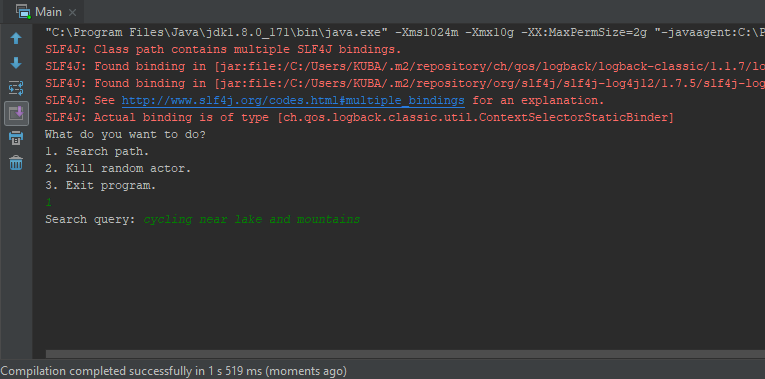
\includegraphics[width=\textwidth]{SS-search.png}
\caption{Zrzut ekranu z konsoli -- szukanie tekstu.}
\label{fig:search}
\end{figure}

Wynik z poszukiwania to wypisanie wszystkich tekstów, które zostały uznane za zgodne z zapytaniem użytkownika. Rysunek \ref{fig:result} prezentuje wycinek z konsoli, na którym widać przykładowy tekst. Można zauważyć, że początek i koniec tekstu z opisem ścieżki odznacza się wielokrotnymi znakami gwiazdki (*). Do każdego tekstu jest także zwrócony \textit{rating}, czyli bliskość tekstu do zapytania. Tekst, który widnieje na zrzucie ekranu posiada wielokrotne odniesienia do jezior i gór oraz opisuje ścieżkę rowerową. Mimo to uzyskał notę jedynie 0.63. Przy dłuższych zapytaniach te noty są coraz niższe, ale wyszukane teksty coraz dokładniej opisują to, czego szuka użytkownik.

\FloatBarrier

\begin{figure}[h!]
\centering
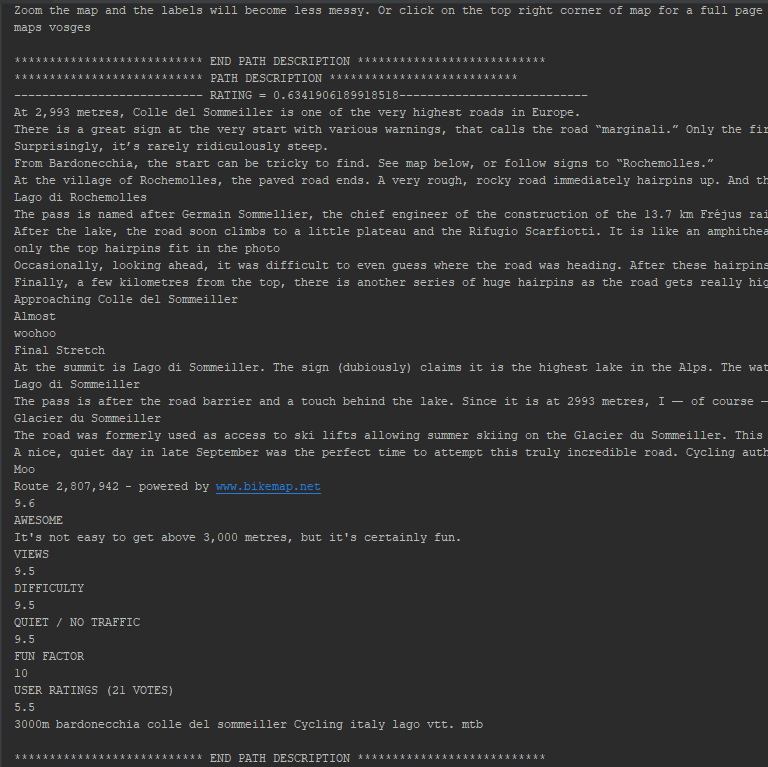
\includegraphics[width=\textwidth]{SS-result.png}
\caption{Zrzut ekranu z konsoli -- wynik szukania tekstu.}
\label{fig:result}
\end{figure}

\FloatBarrier

Użytkownik posiada też możliwość zabicia losowego aktora w celu weryfikacji braku \textit{single point of failure} w systemie. W takim przypadku agent zostanie zabity i użytkownik nie będzie mógł uzyskać od niego informacji, ale nadal będą działały inne agenty, więc system będzie pełnił swoją rolę.

\section{Podsumowanie}

W ramach projektu z przedmiotów \textit{Systemy agentowe [SAG]} oraz \textit{Wprowadzenie do eksploracji danych tekstowych w środowisku www [WEDT]} udało się stworzyć działający system, który umożliwia automatyczne znajdowanie opisów ścieżek sportowych w Internecie. Wyróżnione zostały trzy kategorie sportów: hiking, kolarstwo oraz bieganie z racji ich popularności. Bardzo pomocne przy projektowaniu systemu było skorzystanie z architektury aktorowej i frameworka Akka. Pozwoliło to w bardzo łatwy sposób na zaprojektowanie rozproszonego systemu, bez \textit{single point of failure}, który również działał szybko i sprawnie z powodu zastosowania komunikacji asynchronicznej. Stworzony przez nas system mógłby być dobrym prototypem dla rzeczywistego serwisu internetowego, który umożliwiałby wyszukiwanie tras biegowych/wycieczkowych/kolarskich.


\end{document}
